\chapter{Implementação}
\label{cap:implementacao}

O protótipo AppMan ainda está em desenvolvimento, portanto nem todos os requisitos descritos no modelo GRAND constam no protótipo e, seu funcionamento ainda apresenta alguns comportamentos inesperados. 

Desenvolvido com seu código fonte aberto, seus fontes estão em um repositório acessível para qualquer um que deseja visualizá-los.

Este trabalho foi desenvolvido usando como base arquivos existente em um \emph{branch} do repositório svn que o AppMan se encontra. De acordo com a documentação contida nestes arquivos, eles já possuem uma integração através do uso da DRMAA. Ao testar esses arquivos esta versão não estava funcional. Alguns ajustes, que serão explicados posteriormente, foram necessários para o funcionamento correto desta versão.

\section{Criação do Ambiente Computacional}

Para o desenvolvimento do trabalho proposto foi criado um ambiente computacional com um RMS OpenPBS instalado possuindo três nós para submissão de tarefas. Foi configurado um servidor LDAP necessário para a execução do middleware EXEHDA/ISAM. A instalação do OpenPBS foi feito em um computador com processador AMD Turion(tm) 64 X2 Mobile Technology TL-50 1.6Ghz e 1.5Gb de memória RAM. O Servidor LDAP foi instalando em um computador AMD Athlon(tm) 64 X2 Dual Core Processor 4000+ 2.2Ghz e memório RAM de 2.0Gb. Este computador também está na lista de nós do OpenPBS além de mais dois outros. O primeiro possui processador AMD Sempron(tm) 2500+ 1.8Ghz e memória RAM de 512Mb e o outro possui um processador Intel(R) Celeron(R) 2.00GHz com 512Mb de memória RAM. Em todos os computadores o sistema operacional é Linux Ubuntu 7.10 com Kernel 2.6.22.

Para compilação e alterações nos fontes do protótipo foi usado as IDEs NetBeans\cite{netbeans} e Eclipse\cite{eclipse}, para geração de diagramas UML bem como a engenharia reversa do AppMan, foi usado, além das IDEs citadas, o software Umbrello\cite{umbrello}.

\section{Componente DRMAA (submissão e monitoração)}

Baseado na implementação desenvolveu-se um modelo definido por um conjunto de classes conforme figura 6.1. Os principais métodos necessários para submissão e monitoração de uma tarefa estão na classe \emph{appman.rmswrapper.pbs.drmaa.SessionImpl} que implementa a \emph{interface} \emph{org.ggf.drmaa.Session}.

A DRMAA java \emph{binding} foi implementada com a JAVA \emph{Native Interface} (JNI). JNI é uma \emph{interface} de padrão de programação para escrever métodos Java sob uma máquina virtual Java (JVM), fazendo chamadas recebendo chamadas de aplicações nativas. Essas aplicações nativas, são aplicações específicas do sistema operacional. Dentre as linguagens, pode-se fazer chamadas em C++, C e \emph{Assembly} \cite{jni}.

\begin{figure}[htb]
\begin{center}
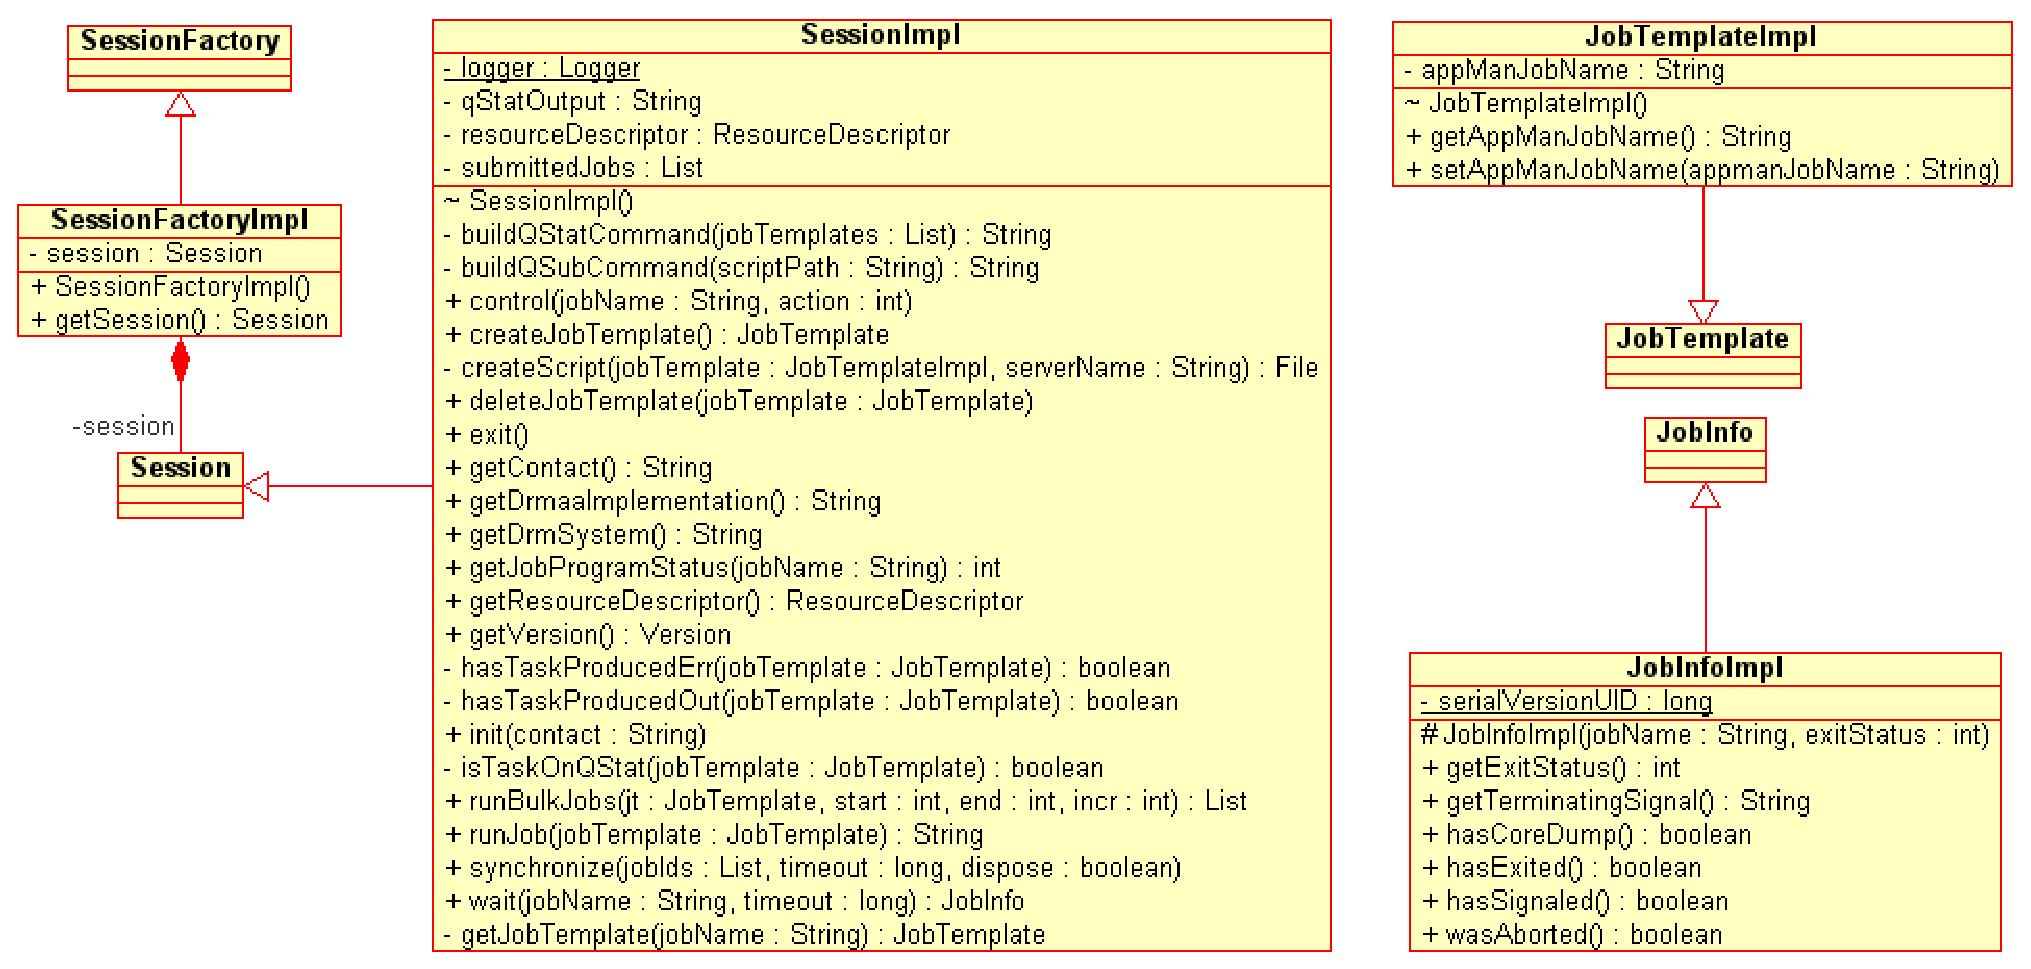
\includegraphics[scale=0.5]{./img/drmaaUML2.eps}
\caption{Diagrama de classes do pacote \textbf{appman.rmswrapper.pbs.drmaa}}
\label{fig:UML_DRMAA}
\end{center}
\end{figure}

Dentre os inúmeros métodos existentes na classe \emph{SessionImpl} os mais relevantes para o AppMan são:

\begin{itemize}
	\item \emph{String runJob(JobTemplate jobTemplate)} submete uma tarefa e tem como retorno um identificador para ser usado se necessário.
	\item \emph{JobInfo wait(String jobName, long timeout)} espera o final da execução por um determinado tempo máximo.
	\item \emph{appman.rmswrapper.pbs.drmaa.JobTemplateImpl} encapsula a definição de uma tarefa para submissão.
	\item \emph{appman.rmswrapper.pbs.drmaa.JobInfoImp} representa a tarefa após a sua execução.
\end{itemize}

\section{AppMan com DRMAA}

Conforme análise do código encontrado no repositório, a integração ficou concentrada em duas mudanças. A primeira é a criação de uma classe nova \emph{appman.GridTaskDrmaa} e a outra foi uma alteração no arquivo de configuração que indica em qual componente é responsável para executação da tarefa, ou \emph{middleware} EXEHDA, ou nova implementação. Com isso, o impacto da modificação torna-se relativamente baixo. 

\subsection{Classe GridTaskDrmaa}

A nova classe implementa a mesma \emph{interface} que a classe padrão \emph{appman.GridTask}. A maior alteração encontra-se no método \emph{execute} onde são feitas as chamadas ao componente de submissão. O método \emph{execute} figura 6.2, é onde são realizados os passos indicados pela especificação DRMAA na submissão e monitoração de tarefas.

\begin{figure}[htb]
\begin{center}
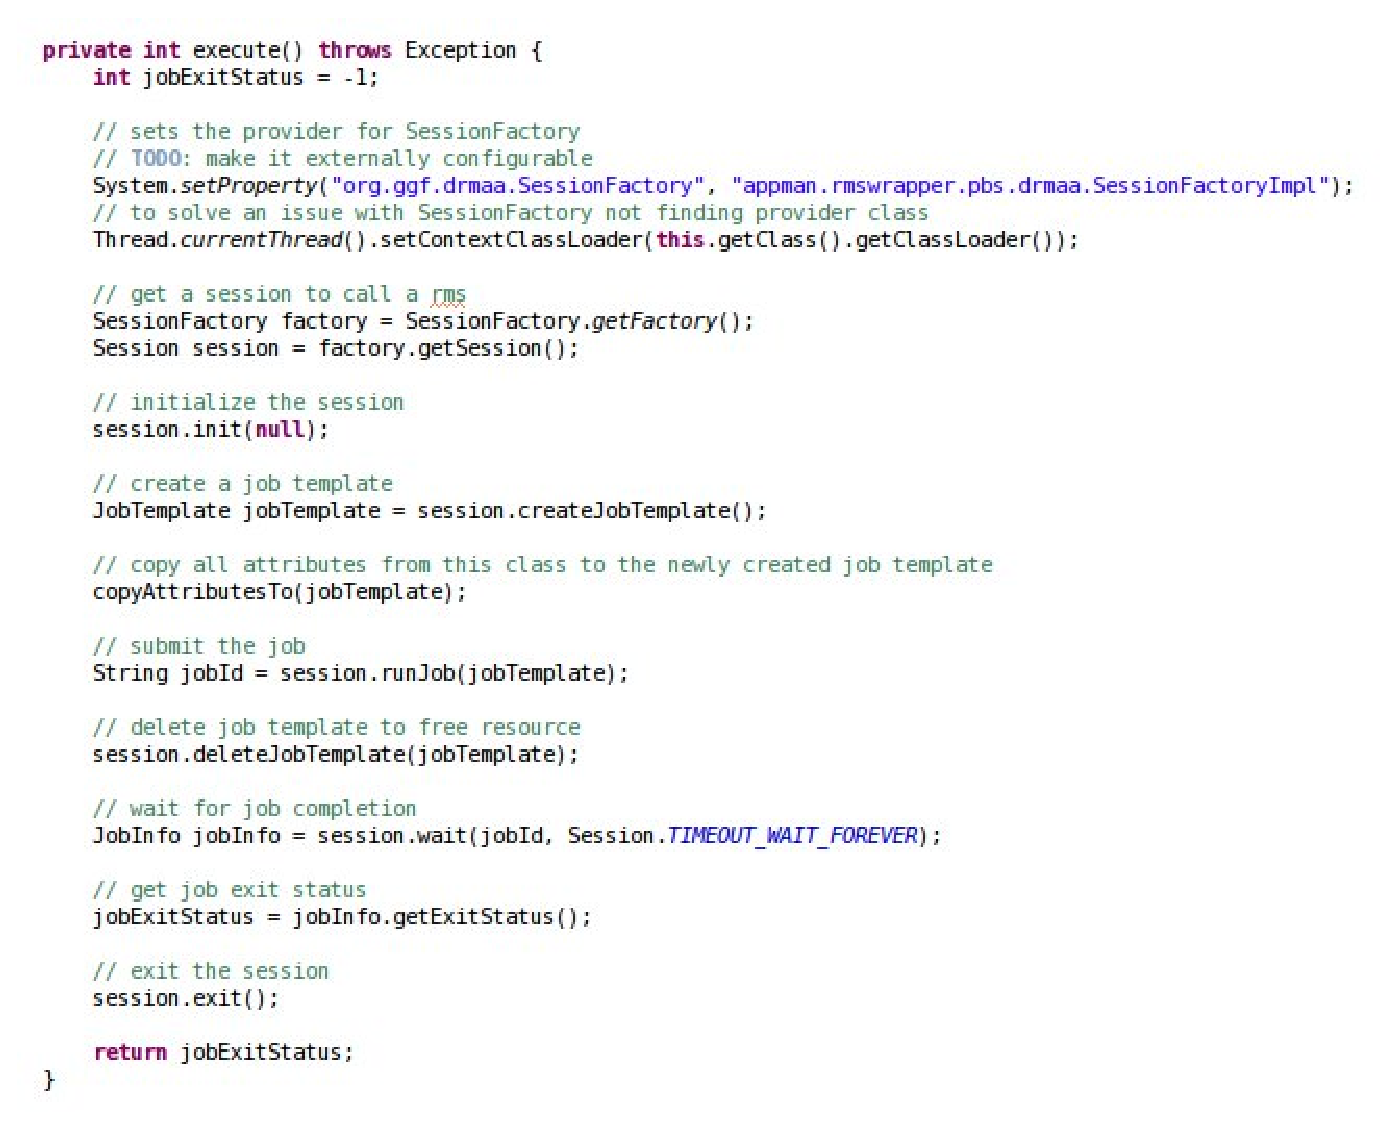
\includegraphics[scale=0.65]{./img/execute.eps}
\caption{Método \emph{execute} da nova classe \emph{appman.GridTaskDrmaa}}
\label{fig:UML_DRMAA}
\end{center}
\end{figure}

\subsection{Arquivo de configuração}

A alteração no arquivo de configuração foi feita para que o nó saiba que componente usar na submissão da tarefa. Esta alteração consiste na criação de uma propriedade que recebe o valor que indica qual componente usar. A figura x exemplifica o arquivo de configuração onde o \emph{Submission Manager} criado no nó \textbf{0.desktop} usará a \emph{GridTaskDrmaa} para submeter tarefas e o nó \textbf{0.notebook} usará \emph{GridTask} para submeter.

\begin{figure}[htb]
\begin{center}
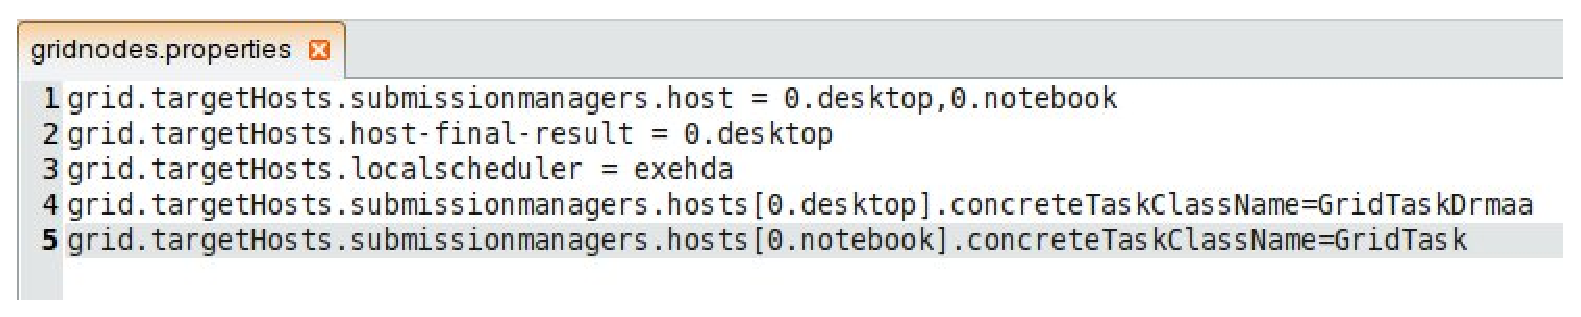
\includegraphics[scale=0.5]{./img/gridnodes_properties.eps}
\caption{Arquivo de configuração \emph{gridnodes.properties}}
\label{fig:gridonodes_properties}
\end{center}
\end{figure}

Para que esta nova configuração fosse reconhecida foi criado o metódo \emph{loadConcreteTaskClassName} na classe \emph{TaskManager} (\textbf{vou colocar uma figura do método}) o qual lê a propriedade no arquivo de configuração e retorna o nome do componente configurado para onde submeter a tarefa. Na implementação atual não foi possível, conforme sugerido, a criação de um \emph{Submission Manager} que submete tarefas via componente DRMAA e um \emph{Submission Manager} usando o componente padrão ao mesmo tempo.